% \documentclass[handout]{beamer}
\documentclass{beamer}
\mode<presentation>
{
  \usetheme{Warsaw}
  % \setbeamercovered{transparent}
  \useoutertheme{infolines}

}

\usepackage[italian]{babel}
\usepackage[utf8]{inputenc}
\usepackage{wrapfig}
\usepackage[T1]{fontenc}
\usepackage{float}
\usepackage{multicol}
\usepackage{pgfplots}
\usepackage{graphicx}
\usepackage{algorithm}
\usepackage{xcolor}
\usepackage{tikz}
\usetikzlibrary{positioning,shapes,chains,backgrounds,arrows,chains,fit,snakes,calc,automata}
\usepackage{array}
\usepackage{subcaption}
\pgfplotsset{compat=1.13}
\usepackage{pdfpages}
\newcolumntype{P}[1]{>{\centering\arraybackslash}p{#1}}
\usepackage{algorithm}
\usepackage[noend]{algpseudocode}
\usepackage{blindtext}
\usepackage{mwe}
\usepackage{tikz}\usetikzlibrary{er}\tikzset{multi  attribute /.style={attribute
    ,double  distance =1.5pt}}\tikzset{derived  attribute /.style={attribute
    ,dashed}}\tikzset{total /.style={double  distance =1.5pt}}\tikzset{every
  entity /.style={draw=orange , fill=orange!20}}\tikzset{every  attribute
  /.style={draw=MediumPurple1, fill=MediumPurple1!20}}\tikzset{every
  relationship /.style={draw=Chartreuse2,
    fill=Chartreuse2!20}}\newcommand{\key}[1]{\underline{#1}}
\usetikzlibrary{arrows.meta}
\usetikzlibrary{decorations.markings}
\usetikzlibrary{arrows,shapes,backgrounds,petri} 
\usetikzlibrary{automata,positioning}
\usetikzlibrary{matrix}

\definecolor{nord1}{RGB}{46, 52, 64}
\definecolor{nord2}{RGB}{76, 105, 141}
\definecolor{nord3}{RGB}{94, 129, 172}
\definecolor{nord4}{RGB}{129, 161, 193}
\definecolor{nord5}{RGB}{136, 192, 208}
\definecolor{nord6}{RGB}{163, 190, 140}
\definecolor{nord7}{RGB}{191, 97, 106}
\definecolor{nordred}{RGB}{191, 97, 106}
\definecolor{nordgreen}{RGB}{135, 157, 116}

\setbeamercolor{palette primary}{bg=nord2,fg=white}
\setbeamercolor{palette secondary}{bg=nord3,fg=white}
\setbeamercolor{palette tertiary}{bg=nord4,fg=white}


\setbeamercolor{block title}{bg=nord2,fg=white}

\setbeamercolor{itemize item}{fg=nord3}
\setbeamercolor{itemize subitem}{fg=nord4}
\setbeamercolor{itemize subsubitem}{fg=nord5}

\setbeamertemplate{itemize item}[square]
\setbeamertemplate{itemize subitem}[circle]
\setbeamertemplate{itemize subsubitem}[triangle]
\setbeamerfont{bibliography item}{size=\scriptsize}
\setbeamerfont{bibliography entry author}{size=\scriptsize}
\setbeamerfont{bibliography entry title}{size=\scriptsize}
\setbeamerfont{bibliography entry location}{size=\tiny}
\setbeamerfont{bibliography entry note}{size=\tiny}

\usecolortheme[named=nord2]{structure}
\setbeamertemplate{bibliography item}{\insertbiblabel}
\def\SLP{\mbox{\rm {\sf SLP}}}
\def\rank{\mbox{\rm {\sf rank}}}
\def\lcs{\mbox{\rm {\sf lcs}}}
\def\lcp{\mbox{\rm {\sf lcp}}}
\def\lce{\mbox{\rm {\sf lce}}}
\def\LCE{\mbox{\rm {\sf LCE}}}
\def\ROT{\mbox{\rm {\sf ROT}}}
\def\select{\mbox{\rm {\sf select}}}
\def\col{\mbox{\rm {\sf col}}}
\def\NULL{\mbox{\rm {\sf null}}}
\def\len{\mbox{\rm {\sf len}}}
\def\pos{\mbox{\rm {\sf pos}}}
\def\row{\mbox{\rm {\sf row}}}
\def\LF{\mbox{\rm {\sf LF}}}
\def\FL{\mbox{\rm {\sf FL}}}
\def\W{\mbox{\rm {\sf w}}}
\def\A{\mbox{\rm {\sf A}}}
\def\A{\mbox{\rm {\sf A}}}
\def\SA{\mbox{\rm {\sf SA}}}
\def\LCP{\mbox{\rm {\sf LCP}}}
\def\ISA{\mbox{\rm {\sf ISA}}}
\def\PLCP{\mbox{\rm {\sf PLCP}}}
\def\RLCP{\mbox{\rm {\sf RLCP}}}
\def\RLBWT{\mbox{\rm {\sf RLBWT}}}
\def\MEM{\mbox{\rm {\sf MEM}}}
\def\KMEM{\mbox{\rm {\sf K-MEM}}}
\def\KSMEM{\mbox{\rm {\sf K-SMEM}}}
\def\MS{\mbox{\rm {\sf MS}}}
\def\LCP{\mbox{\rm {\sf LCP}}}
\def\NSV{\mbox{\rm {\sf NSV}}}
\def\PSV{\mbox{\rm {\sf PSV}}}
\def\RMQ{\mbox{\rm {\sf RMQ}}}
\def\BWT{\mbox{\rm {\sf BWT}}}
\def\BWM{\mbox{\rm {\sf BWM}}}
\def\ITR{\mbox{\rm {\sf index\_to\_run}}}
\def\GS{\mbox{\rm {\sf get\_symbol}}}
\def\PBWT{\mbox{\rm {\sf PBWT}}}
\def\MPBWT{\mbox{\rm {\sf mPBWT}}}
\def\MRLPBWT{\mbox{\rm {\sf mRLPBWT}}}
\def\DPBWT{\mbox{\rm {\sf dPBWT}}}
\def\RLPBWT{\mbox{\rm {\sf RLPBWT}}}
\def\SMEM{\mbox{\rm {\sf SMEM}}}
\def\M{\mbox{\rm {\sf M}}}
\def\C{\mbox{\rm {\sf C}}}
\def\Occ{\mbox{\rm {\sf Occ}}}
\def\L{\mbox{\rm {\sf L}}}
\def\F{\mbox{\rm {\sf F}}}
\def\DA{\mbox{\rm {\sf DA}}}
\def\DM{\mbox{\rm {\sf DM}}}
\def\PA{\mbox{\rm {\sf PA}}}
\def\LCE{\mbox{\rm {\sf LCE}}}
\def\UP{\mbox{\rm {\sf update}}}
\def\lceb{\mbox{\rm {\sf lce\_bounded}}}
\def\RM{\mbox{\rm {\sf reverse\_map}}}

\newcommand{\Oh}{\mathcal{O}}

\title[] {Algoritmi per la trasformata di Burrows-Wheeler posizionale con
  compressione run-length}

% \subtitle
% {Presentation Subtitle} % (optional)

\author[1]{\Large{Davide Cozzi}}


\institute[] {\large{\textbf{{\color{nord2}Relatore:}} \textit{Prof.~Raffaella
      Rizzi}\quad 
    \textbf{\color{nord2}{Correlatore:}} \textit{Dr.~Yuri Pirola}}\\
  \vspace{4mm}
  \small{\textit{Dipartimento di Informatica, Sistemistica e Comunicazione
      (DISCo)\\
      Università degli Studi di Milano Bicocca}}}

\date[] {25 Ottobre 2022}

\subject{Presentatazione}
\pgfdeclareimage[height=0.5cm]{university-logo}{img/logo_unimib.pdf}
\logo{\pgfuseimage{university-logo}}

\AtBeginSection[]
{
  \begin{frame}<beamer>{Outline}
    \tableofcontents[currentsection, currentsubsection]
  \end{frame}
}


% If you wish to uncover everything in a step-wise fashion, uncomment
% the following command: 

% \beamerdefaultoverlayspecification{<+->}


\begin{document}

\begin{frame}
  \titlepage
\end{frame}

\begin{frame}{Outline}
  \setcounter{tocdepth}{1}
  \tableofcontents
\end{frame}
\section{Introduzione}
\subsection{Pangenoma e aplotipi}
\begin{frame}{Un punto di vista per il pangenoma}
  \begin{block}{}
    Negli ultimi anni si è assistito a un cambio di paradigma nel campo della
    \textit{bioinformatica}, ovvero il passaggio dallo studio della sequenza
    lineare di 
    un singolo genoma a quello di un insieme di genomi, provenienti da un gran
    numero di individui, al fine di poter considerare anche le varianti geniche.
    Questo nuovo concetto è stato introdotto da Tettelin, nel 2005, con il
    termine di \textbf{pangenoma}. 
  \end{block}
  \pause
  \begin{block}{}
    Uno degli approcci più usati per rappresentare il \textbf{pangenoma}
    è attraverso un pannello di aplotipi, ovvero, da un punto di vista
    computazionale, una matrice di M righe, corrispondenti agli individui, e N
    colonne, corrispondenti ai siti con le varianti. 
  \end{block}
  \pause
  \begin{block}{}
    Un \textbf{aplotipo} è  l'insieme di alleli, ovvero di
    varianti che, a meno di mutazioni, un organismo eredita da ogni genitore. 
  \end{block}
\end{frame}
\section{Preliminari}
% \subsection{Bitvector e straight-line program}
% \begin{frame}[fragile]{BV e SLP}
%   \only<1,2>{
%     \begin{block}{BV}
%       \begin{center}
%         \begin{tikzpicture} [nodes in empty cells,
%           nodes={minimum width=0.6cm, minimum height=0.6cm},
%           row sep=-\pgflinewidth, column sep=-\pgflinewidth,ampersand replacement=\&]
%           border/.style={draw}
          
%           \matrix(vector)[matrix of nodes,
%           row 1/.style={nodes={draw=none, minimum width=0.3cm}},
%           nodes={draw}]
%           {
%             \tiny{0} \& \tiny{1} \& \tiny{2} \& \tiny{3} \& \tiny{4} \& \tiny{5}\&\tiny{6}
%             \& \tiny{7} \& \tiny{8} \& \tiny{9} \& \tiny{10} \& \tiny{11} \& \tiny{12} \&
%             \tiny{13}\\  
%             $\mathbf{1}$ \& $0$ \& $0$ \& $\mathbf{1}$ \& $0$ \& $\mathbf{1}$ \& $0$ \&
%             $\mathbf{1}$ \& $0$ \& $\mathbf{1}$ \& $0$ \& $0$ \& $\mathbf{1}$ \& $0$\\ 
%           };
%         \end{tikzpicture}
%       \end{center}
%       \[\mathtt{rank}(6)=3\quad\quad\mathtt{select}(5) =9\]
%     \end{block}
%     \pause
%     \begin{block}{SLP}
%       \[s=\mbox{GATTAGATACAT}\$\mbox{GATTACATAGAT}\]
%       \[\mbox{S}\to \mbox{ZWAY}\,\$\mbox{ZYAW}\]
%       \vspace{-8mm}
%       \begin{multicols*}{5}
%         \small
%         \begin{itemize}
%           \item $\mbox{Z}\to \mbox{WX}$
%           \item $\mbox{Y}\to \mbox{CV}$
%           \item $\mbox{X}\to \mbox{TA}$
%           \item $\mbox{W}\to \mbox{GV}$
%           \item $\mbox{V}\to \mbox{AT}$
%         \end{itemize}
%       \end{multicols*}
%     \end{block}
%   }\only<3>{
%     \begin{block}{SLP}
%       \begin{figure}[H]
%         \centering
%         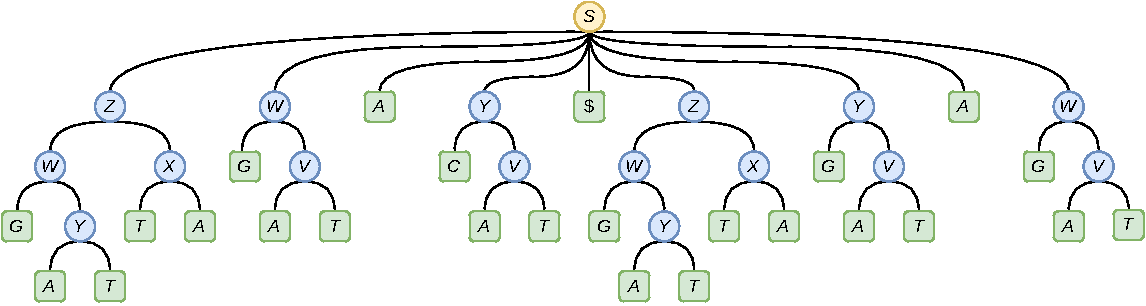
\includegraphics[width=\textwidth]{img/slpgagie.pdf}
%       \end{figure}
%     \end{block}
%   }
% \end{frame}
%\subsection{Trasformata di Burrows-Wheeler, suffix array e maximal exact matches} 
\subsection{Run-length encoded BWT}
\begin{frame}{RLBWT}
    \begin{block}{Esempio\cite{rlpbwt}}
      \begin{table}
        \scriptsize
        \begin{tabular}{ P{0.5cm}|P{0.5cm}|P{0.4cm}|P{1.5cm}|P{0.65cm}|P{1.4cm}|P{0.6cm}|P{2.8cm}  }
          \hline
          \multicolumn{2}{c|}{Thresholds} & &  &  &  & &  \\
          \hline
          {\tt A} & {\tt T}   & $\SA$ & $\SA$ sample  & $\BWT$    & Run heads & $\LCP$ & $\mathcal{M}$ \\
          \hline
                                          &           & 15    & 15           & {\tt A}   & {\tt A}   & 0 & {\tt \$ATTAGATTACATTA} \\
          *     &           & 14    & 14           & {\tt T}   & {\tt T}   & 0 & {\tt A\$ATTAGATTACATT} \\
                                          &            & 9     &              & {\tt T}   &           & 1 & {\tt ACATTA\$ATTAGATT} \\
                                          &            & 4     &              & {\tt T}   &           & 1 & {\tt AGATTACATTA\$ATT} \\
                                          &           & 11    & 11            & {\tt C}   & {\tt C}   & 1 & {\tt ATTA\$ATTAGATTAC} \\
                                          &           & 6     & 6             & {\tt G}   & {\tt G}   & 4 & {\tt ATTACATTA\$ATTAG} \\
                                          &           & 1     & 1             & {\tt \$}  & {\tt \$}  & 4 & {\tt ATTAGATTACATTA\$} \\
                                          &    *       & 10    & 10            & {\tt A}   & {\tt A}   & 0 & {\tt CATTA\$ATTAGATTA} \\
                                          &           & 5     &               & {\tt A}   &          & 0 & {\tt GATTACATTA\$ATTA} \\
          *     &           & 13    & 13            & {\tt T}   & {\tt T}   & 0 & {\tt TA\$ATTAGATTACAT} \\
                                          &           & 8     &               & {\tt T}   &           & 2 & {\tt TACATTA\$ATTAGAT} \\
                                          &           & 3     &               & {\tt T}   &           & 2 & {\tt TAGATTACATTA\$AT} \\
                                          &           & 12    & 12            & {\tt A}   & {\tt A}   & 1 & {\tt TTA\$ATTAGATTACA} \\
                                          &           & 7     &               & {\tt A}  &           & 3 & {\tt TTACATTA\$ATTAGA} \\
                                          &           & 2     &               & {\tt A}  &           & 3 & {\tt TTAGATTACATTA\$A} \\  
          \hline
        \end{tabular}
      \end{table}
    \end{block}
  
\end{frame}
\subsection{Matching statistics e maximal exact matches} 
% \begin{frame}{MS e MEM}
%   \begin{block}{MS}
%       \footnotesize
%       Dato un testo $T$, con $|T|=n$, e un pattern $P$, con $|P|=m$, si
%       definisce \textbf{matching statistics} di $P$ su $T$ un array $MS$ di
%       coppie $(pos, len)$, lungo quanto il pattern, tale che:
%       \begin{itemize}
%         \item $T[MS[i].pos,MS[i].pos+MS[i].len-1]=P[i,i+MS[i].len-1]$, quindi si
%         ha un match tra $P$ e $T$ lungo $MS[i].len$ a partire da $MS[i].pos$ in
%         $T$ e da $i$ in $P$
%         \item $P[i,i+MS[i].len]$ non occorre in $T$, quindi il match non è
%         ulteriormente estendibile 
%       \end{itemize}
%   \end{block}
%   \pause
%   \begin{block}{MEM}
%       \footnotesize
%       Dato un testo $T$, con $|T|=n$, e un pattern $P$, con $|P|=m$, si definisce
%       una sottostringa $P[i,i+l-1]$, di lunghezza $l$, \textbf{MEM} di $P$ in $T$
%       se:
%       \begin{itemize}
%         \item $P[i,i+l-1]$ è una sottostringa di $T$
%         \item $P[i-1,i+l-1]$ non è una sottostringa di $T$ (non si può estendere a
%         sinistra) e $P[i,i+l]$ non è una sottostringa di $T$ (non si può estendere a
%         destra) 
%       \end{itemize}
%       Un MEM si può calcolare dalle MS:
%       \[MS[i].len=l\land MS[i-1].len\leq MS[i].len\]
%   \end{block}
% \end{frame}
\subsection{Algoritmo di Bannai, MONI e PHONI}
\begin{frame}{MONI e PHONI}
  \begin{block}{MONI}
    \small
    Rossi et al., nel 2021, sfruttarono le conoscenze relative
    alla $\RLBWT$ e all'r-index 
    per ideare \textbf{MONI:\textit{ A Pangenomics Index for Finding MEMs}}
    \cite{moni}. In questa soluzione si ha la costruzione, in due
    sweep, tramite l'uso delle threshold (\textit{algoritmo di
      Bannai}), dell'array delle matching statistics, da cui si computano i
    maximal exact match. 
  \end{block}
  % \pause
  % \begin{block}{LCE}
  %   \small
  %     Dato un testo $T$, tale che $|T|=n$, il risultato della \textbf{LCE query}
  %     tra 
  %     due posizioni $i$ e $j$, tali che $0\leq i,j<n$, corrisponde al più lungo
  %     prefisso comune tra le sotto-stringhe che hanno come indice di partenza
  %     $i$ e 
  %     $j$, avendo quindi il più lungo prefisso comune tra $T[i,n-1]$ e
  %     $T[j,n-1]$. 
  % \end{block}
  \pause
  \begin{block}{PHONI}
    \small
    Nel 2021, Boucher, Gagie, Rossi et al. proposero un ulteriore miglioramento di
    quanto fatto in MONI, con \textbf{PHONI: \textit{Streamed Matching
        Statistics with Multi-Genome References}}\cite{phoni}, usando le
    $\LCE$ query 
    al posto delle threshold.
  \end{block}
\end{frame}
\subsection{Trasformata di Burrows-Wheeler posizionale}
\begin{frame}{PBWT}
  \only<1,2>{
    \begin{block}{Prefix array}
      Dato un aplotipo $i$, appartenente al pannello $X$, e un indice di colonna
      $k$, si definisce il \textbf{prefix array} $a_k$ come una permutazione
      degli indici $0,\ldots, M-1$ tale che $a_k[i]=j$ sse $x_j$ è l'$i$-esimo
      aplotipo di $X$ nell'ordinamento inverso dei prefissi ottenuto alla
      colonna $k$. Quindi $a_k[i]=m$, con $m<M$, altro non è che l'indice della
      sequenza $x_m$ del pannello $X$ da cui deriva il prefisso $i$-esimo
      nell'ordine inverso in colonna $k$.
  \end{block}
  \pause
  \begin{block}{Divergence array}
      Si definisce \textbf{divergence array} l'array $d_k$ tale che $d_k[i]$ è
      l'indice colonna iniziale del match massimale a sinistra terminante in $k$
      tra 
      l'$i$-esimo aplotipo e il suo precedente nell'ordinamento ottenuto alla
      colonna $k$-esima. Formalmente, dato $i>0$, si definisce 
      $d_k[i]$ come il più piccolo $j$ tale che $y_i^k[j,k)=y_{i-1}^k[j,k)$.
      Ne segue che $y_i^k[k-1]\neq y_{i-1}^k[k-1] \implies d_k[i]=k$ (per
      definizione $d_k[0]=k$).
  \end{block}
}\only<3>{
  \begin{block}{}
    \begin{figure}[H]
      \centering
      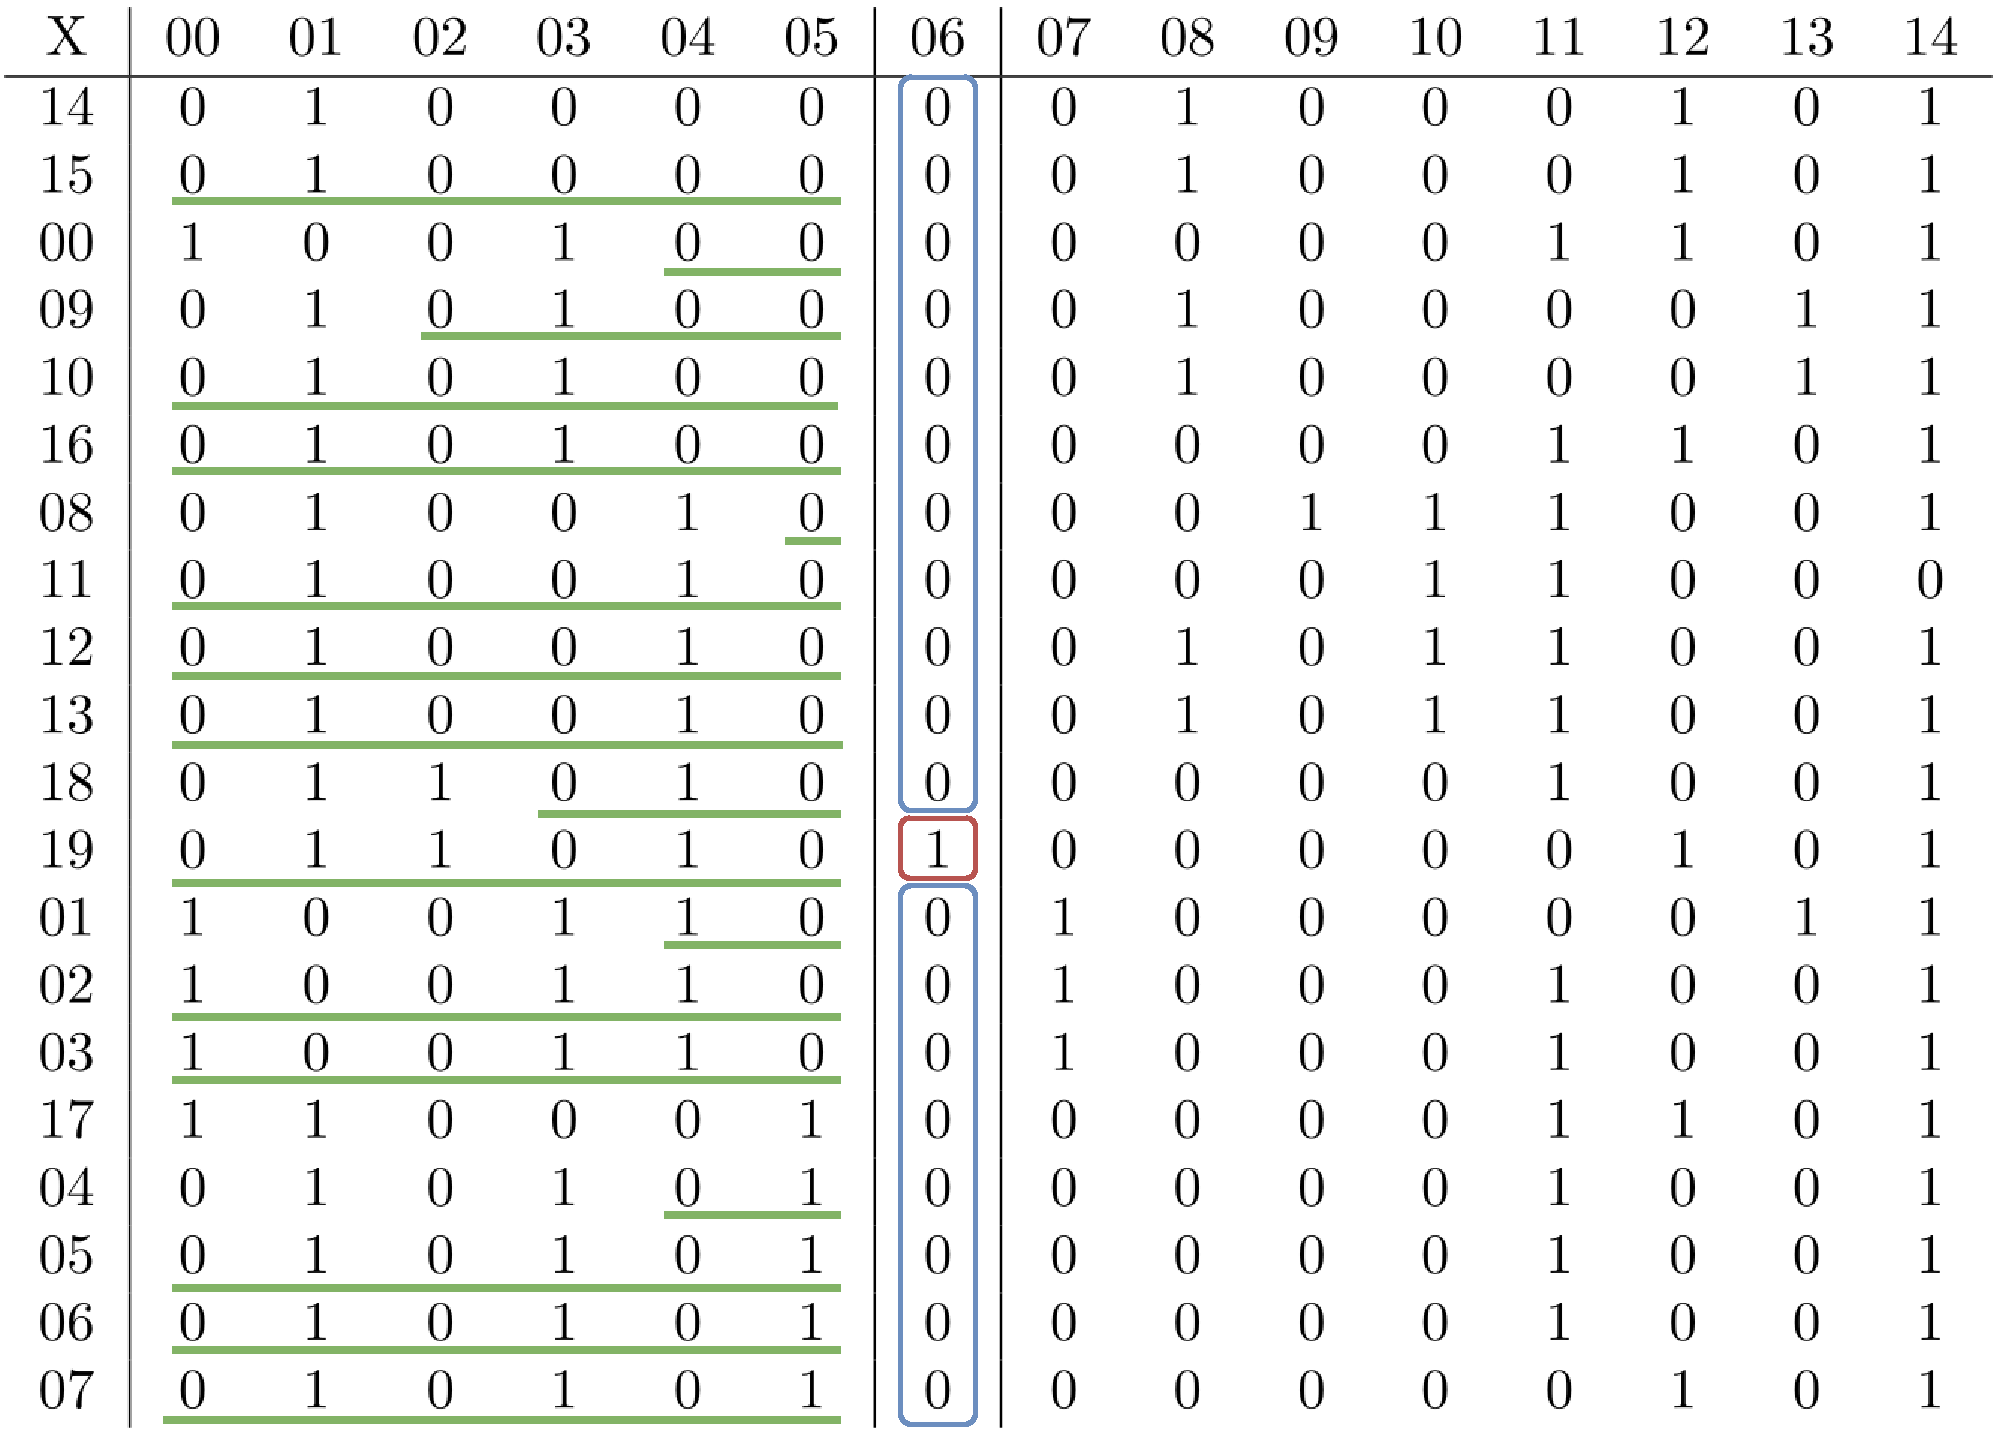
\includegraphics[scale = 0.225]{img/matrix1.pdf}
    \end{figure}
    {\footnotesize{\[a_6=[14,15,0,9,10,16,8,11,12,13,18,19,1,2,3,17,4,5,6,7]\]
    \[d_6=[6,0,4,2,0,0,5,0,0,0,3,0,4,0,0,6,4,0,0,0]\]}}
  \end{block}
}
\end{frame}
\subsection{Set-maximal exact match con la PBWT}
\begin{frame}{Set-maximal exact match}
  \begin{block}{SMEM}
    Dato un pannello $X$, con $M$ aplotipi/righe e $N$ siti/colonne, e un
    aplotipo 
    query $z$, tale che $|z|=N$, si definisce un \textbf{Set-Maximal Exact
      Match}  
      ($\SMEM$), iniziante in colonna $e_k$ e terminante il colonna
    $k$, tra 
    la query $z$ e le righe del pannello indicizzate dai valori compresi
    nell'intervallo $[f_k,g_k)$ in $a_k$ sse:
    \[z[e_k,k)=y_i^k[e_k,k)\land z[e_k-1]\neq y_i^k[e_k-1], \forall\, i\mbox{
        t.c. }f_k\leq i < g_k\]
    Si noti che $g_k=M$ sse $y_{M-1}^k$ appartiene alle righe per le quali si ha
    tale $\SMEM$.
  \end{block}
  \begin{block}{}
    Il calcolo viene effettuato tramite il cosiddetto \textbf{algoritmo 5 di
      Durbin}\cite{pbwt} in tempo Avg.$\mathcal{O}(N+c)$\cite{dpbwt}, avendo $N$
    aplotipi e 
    $c$ $\SMEM$, con una memoria richiesta di 13NM byte.
  \end{block}
\end{frame}
\section{Metodo}
\subsection{Componenti}
\begin{frame}{Componenti e strutture dati}
  \begin{block}{}
    \begin{figure}[H]
      \centering
      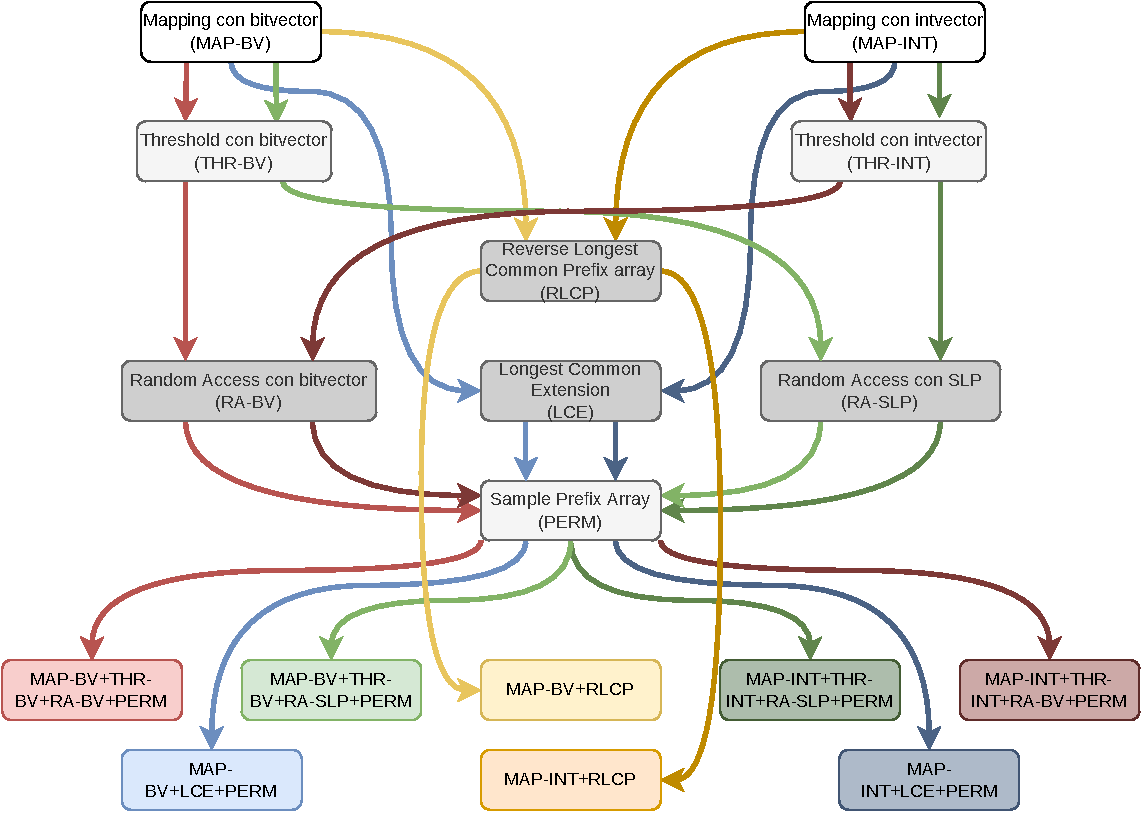
\includegraphics[width=0.85\textwidth]{img/ds.pdf}
    \end{figure}
  \end{block}
\end{frame}
\subsection{Mapping, threshold e prefix array sample}
\subsection{Random access e longest common extension query}
\subsection{Struttura per le funzioni $\varphi$ e $\varphi^{-1}$}
\subsection{Algoritmo di calcolo degli SMEM con LCP}
\subsection{Algoritmo di calcolo degli SMEM con MS}
\section{Risultati sperimentali}
\subsection{1000 Genome Project, ambiente di test e implementazioni}
\subsection{Risultati costruzione strutture}
\begin{frame}{Performance costruzione strutture dati}
  \begin{figure}[H]
    \centering
    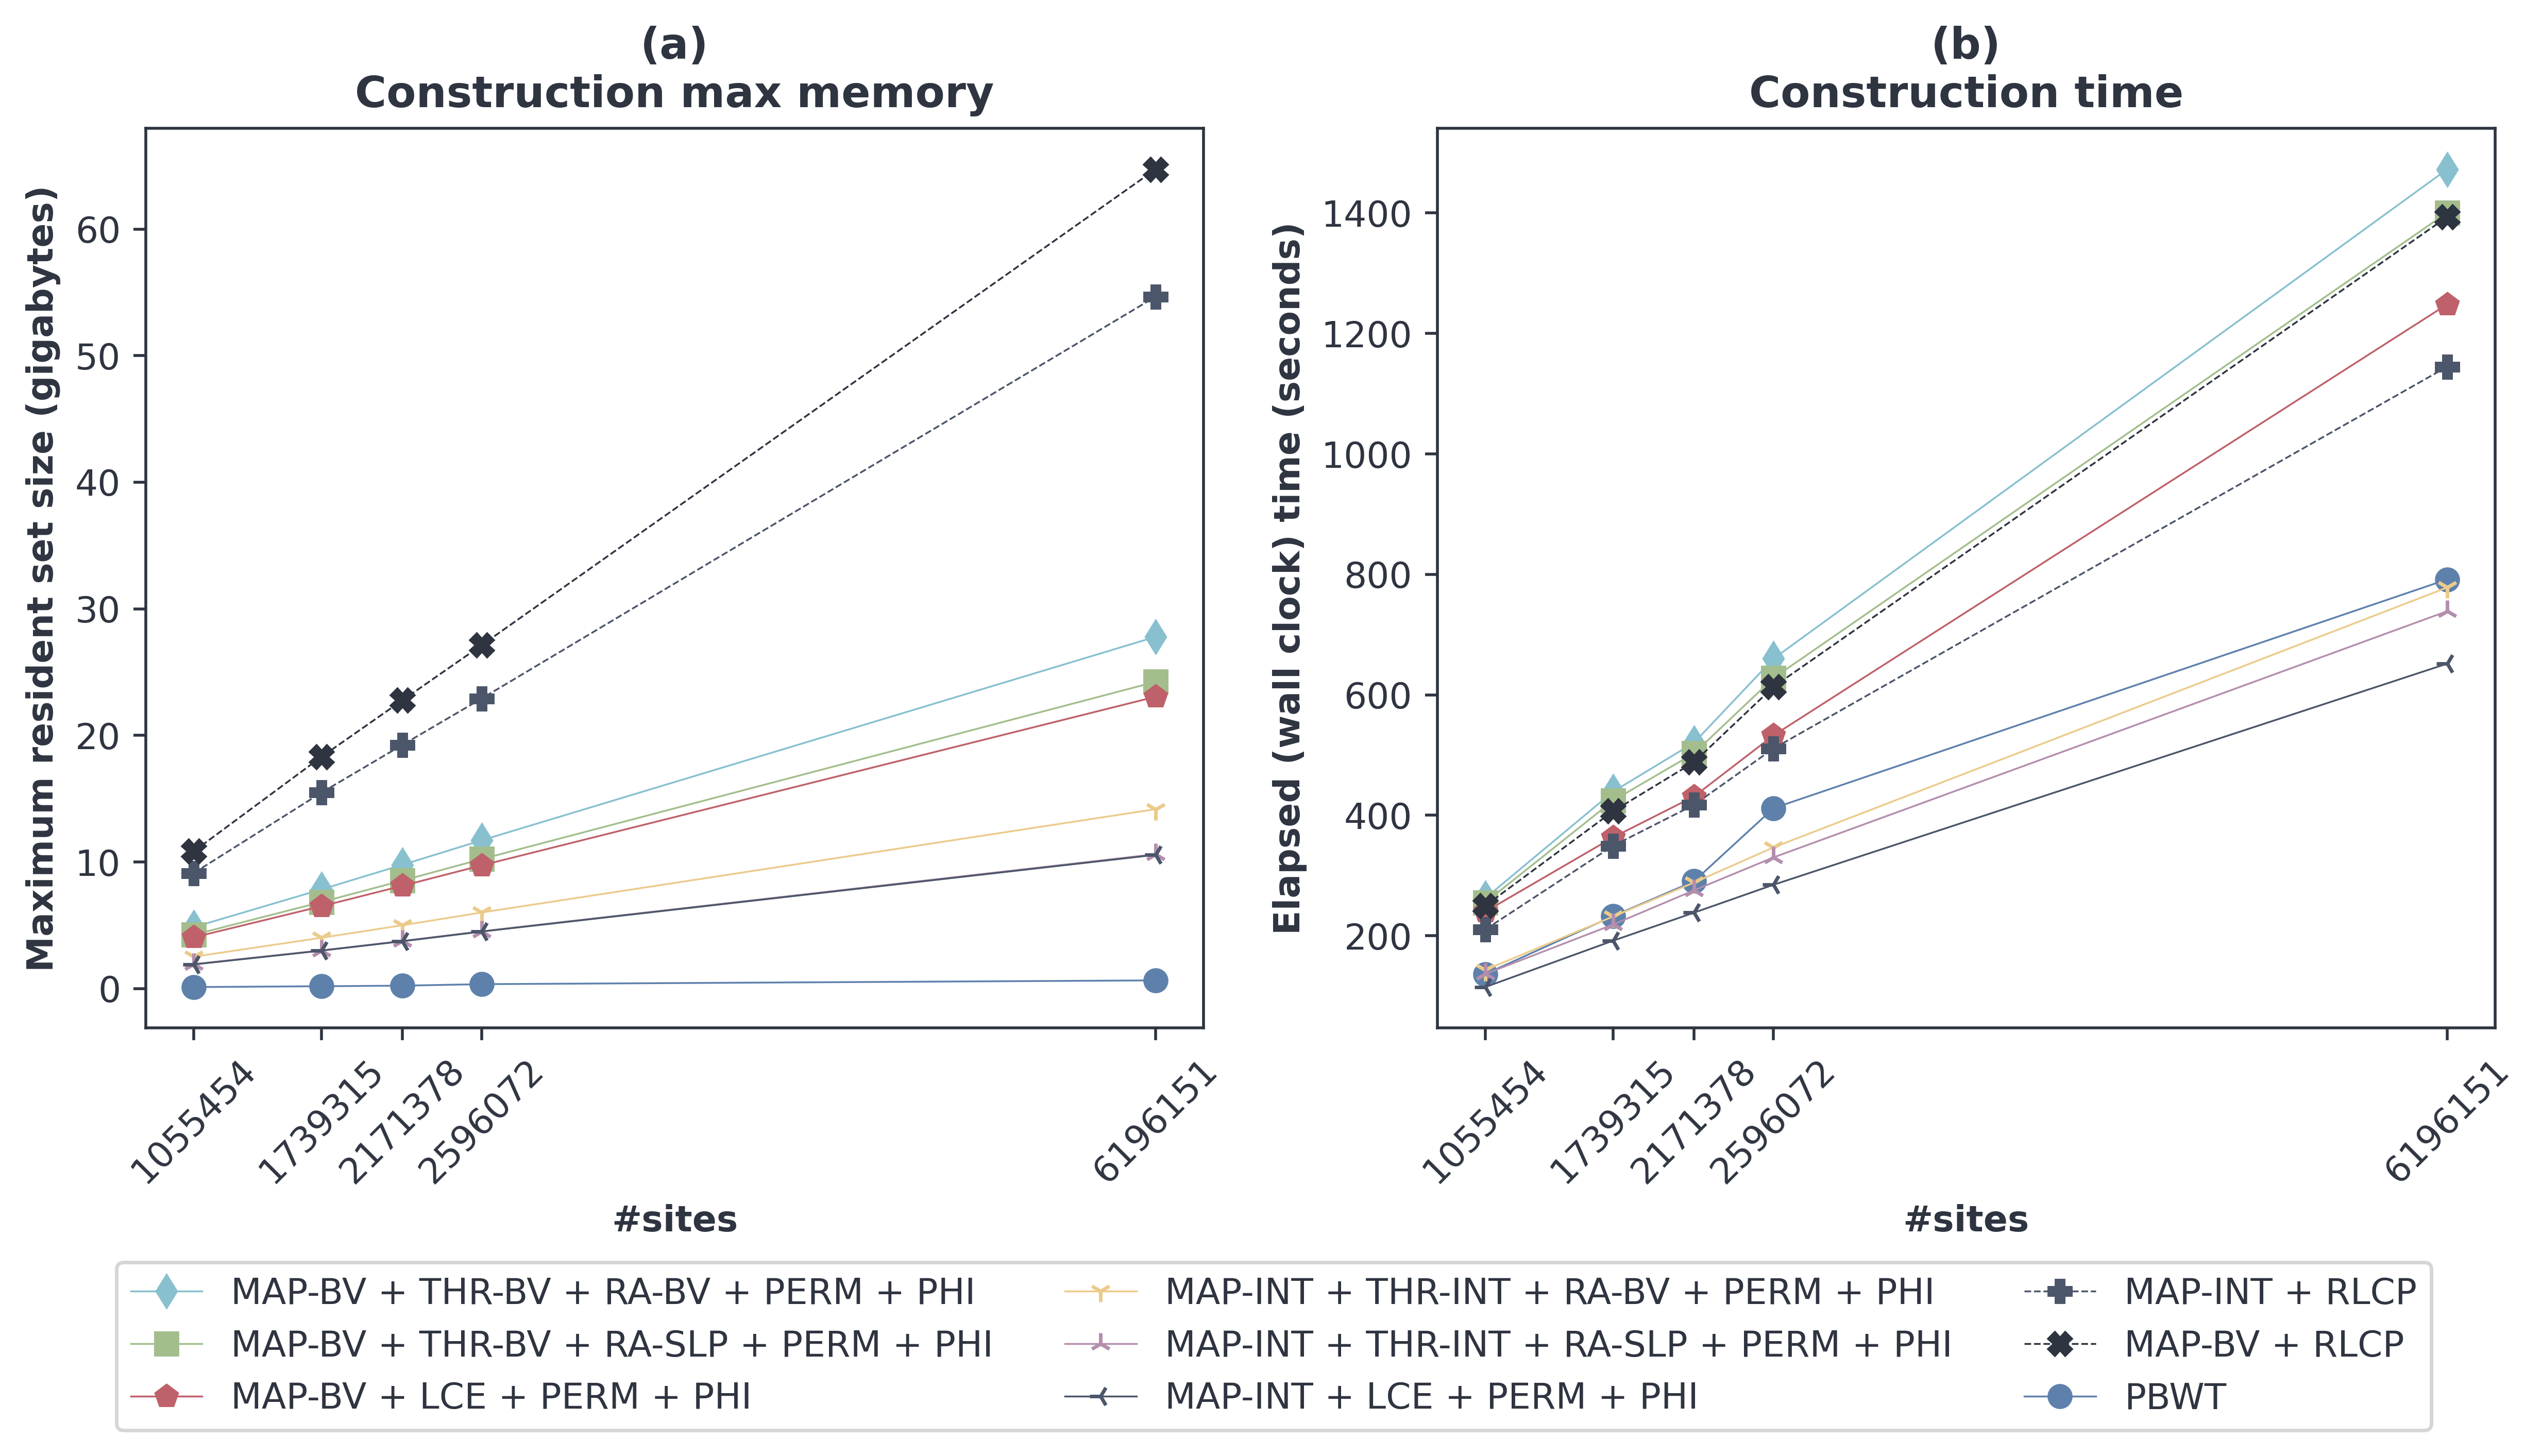
\includegraphics[width=0.9\textwidth]{img/make_time_mem_paper.png}
  \end{figure}
\end{frame}
\subsection{Risultati calcolo degli SMEM}
\begin{frame}{Performance calcolo degli $\SMEM$ con 100 query}
  \begin{figure}[H]
    \centering
    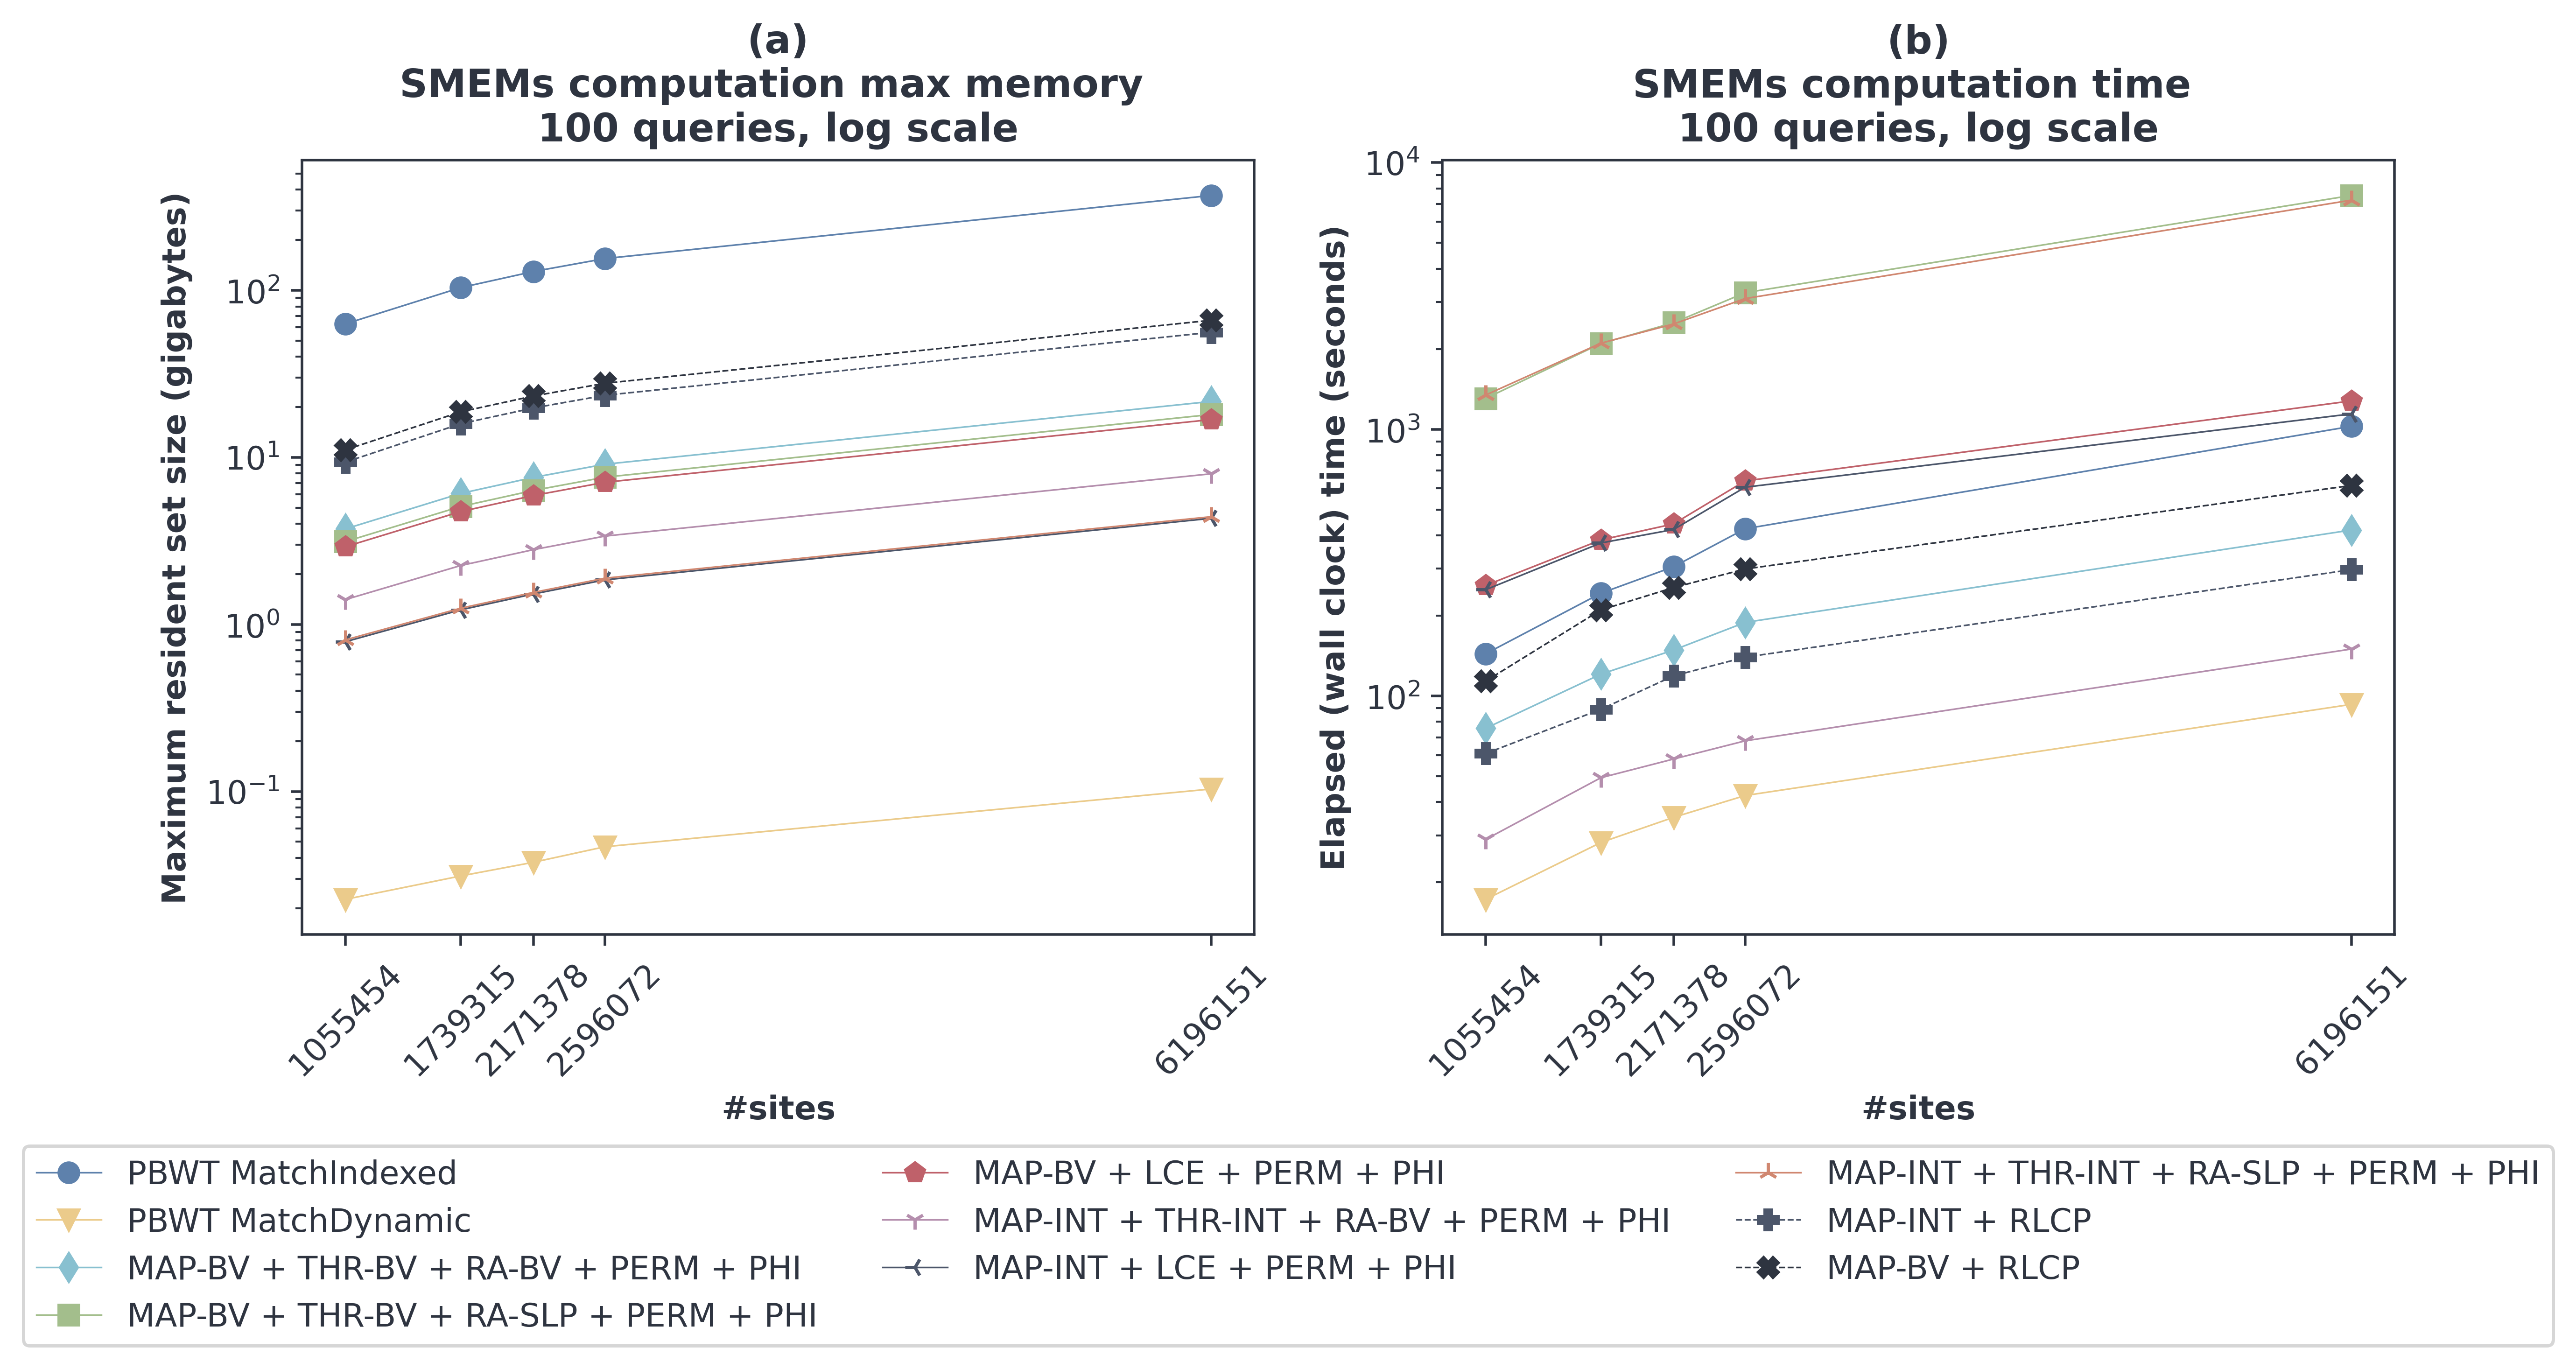
\includegraphics[width=0.9\textwidth]{img/exe_time_mem_paper.png}
  \end{figure}
\end{frame}
\begin{frame}{Performance calcolo degli $\SMEM$ per singole query}
  \begin{figure}[H]
    \centering
    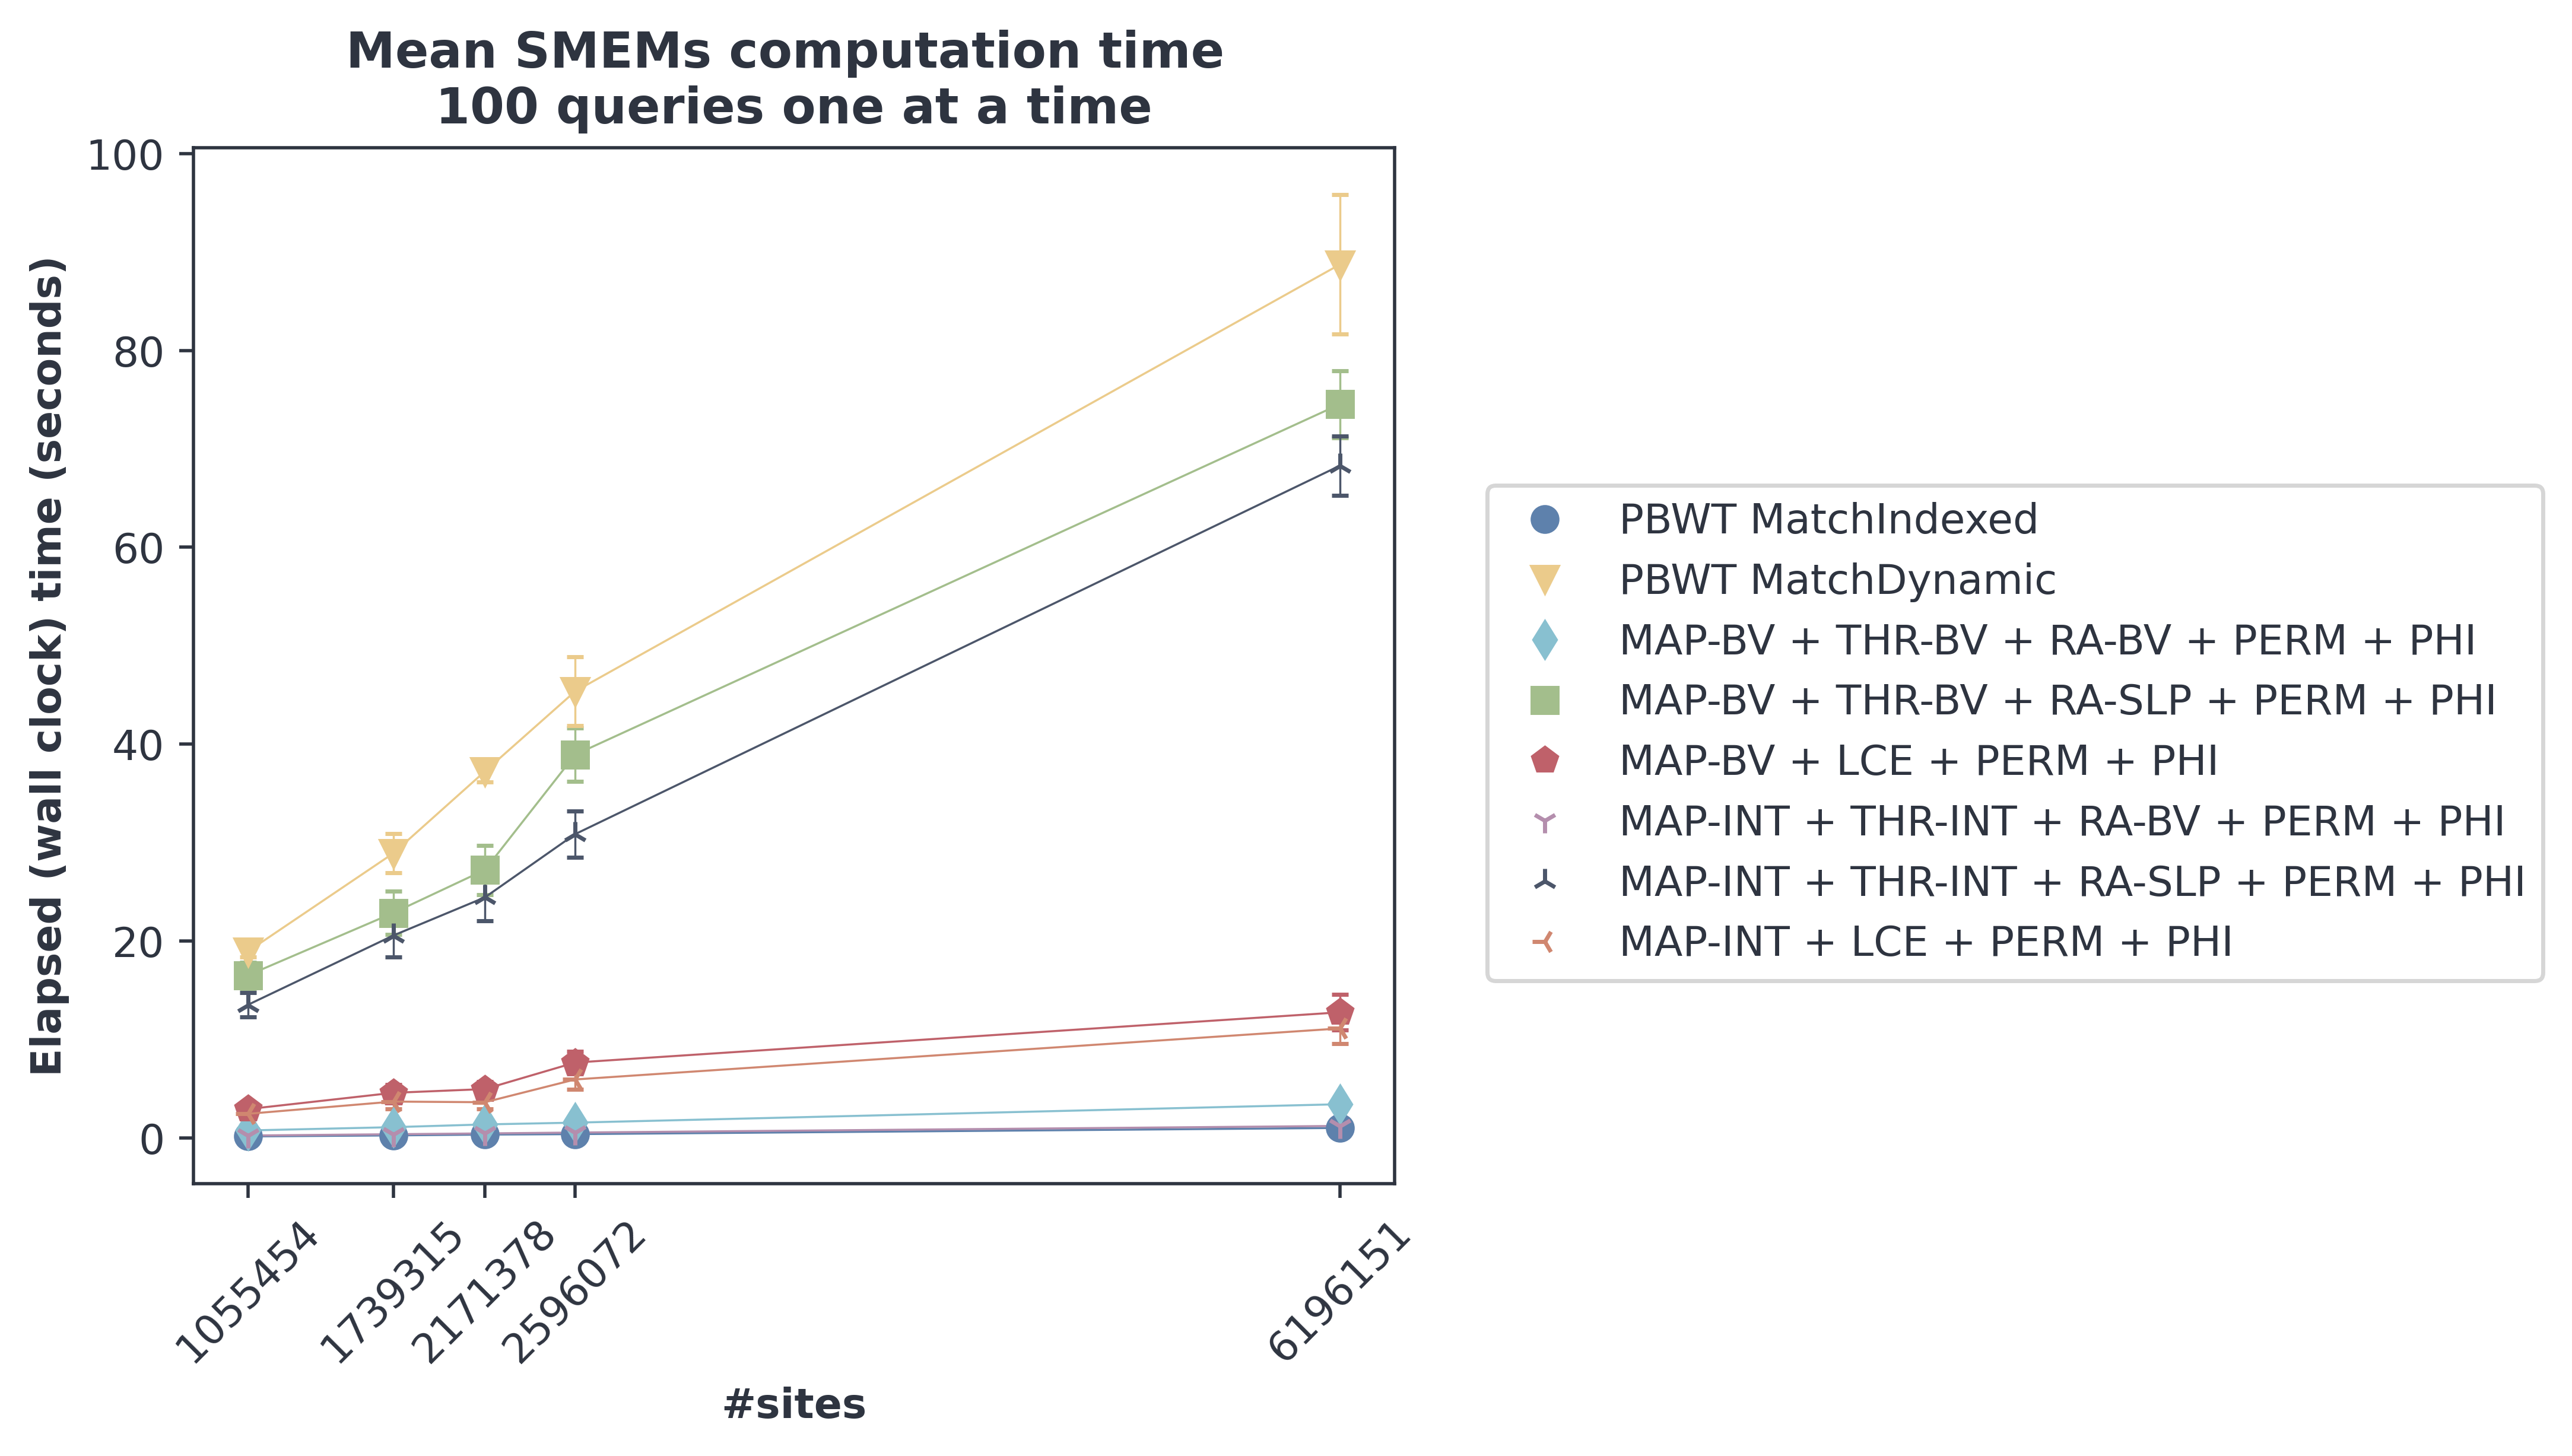
\includegraphics[width=0.9\textwidth]{img/exe_time_single_paper.png}
  \end{figure}
\end{frame}
\section{Conclusioni e sviluppi futuri}
\subsection{Ottimizzazioni, generalizzazioni ed estensioni}
\section{Bibliografia}
\begin{frame}[allowframebreaks]{Bibliografia} 
  \bibliographystyle{unsrt}
  \bibliography{slides}
\end{frame}
\begin{frame}{}
  \setbeamercolor{palette primary}{bg=nord3,fg=white}
  
  \title[] {Grazie per l'attenzione}

  % \subtitle
  % {Presentation Subtitle} % (optional)

  \author[1]{\Large{Davide Cozzi}}


  \institute[] {\large{\textbf{{\color{nord2}Relatore:}} \textit{Prof.~Raffaella
        Rizzi}\quad 
      \textbf{\color{nord2}{Correlatore:}} \textit{Dr.~Yuri Pirola}}\\
    \vspace{4mm}
    \small{\textit{Dipartimento di Informatica, Sistemistica e Comunicazione
        (DISCo)\\
        Università degli Studi di Milano Bicocca}}}

  \maketitle
\end{frame}

\end{document}


